\documentclass[12pt,oneside,a4paper]{article}

\usepackage[backend=biber,style=numeric]{biblatex}
\usepackage{xcolor}
\usepackage{todonotes}
\usepackage{amsmath}
\usepackage{multicol}
\usepackage{caption}
\usepackage{pgfplots}
\usepackage{hyperref}
\usepackage{graphicx}
\graphicspath{{./imgs/}}
\usepackage{listings}
\lstset{
	frame=top,frame=bottom,
	language=C,
	basicstyle=\small\normalfont,
	xleftmargin=\parindent,
	keywordstyle=\color{green!40!black},
	%  commentstyle=\itshape\color{purple!40!black},
	%  identifierstyle=\color{blue},
	%  stringstyle=\color{orange},
	morekeywords={in, globaldata, procedure, input, output, behavior, end, XOR, NOT, AND}, % keyword to highlight
	%  captionpos=t,
	tabsize=2,
	numbers=left,
	stepnumber=1,                   % the step between two line-numbers.        
	numbersep=5pt,
	framexleftmargin=10pt,
	title=\lstname,
	captionpos=t,
	showspaces=false,
}
\DeclareCaptionFormat{listing}{\rule{\dimexpr\textwidth\relax}{0.4pt}\par\vskip1pt#1#2#3}
\captionsetup[lstlisting]{format=listing,singlelinecheck=false, margin=0pt,labelsep=space,labelfont=bf}

\usepackage{booktabs}
\usepackage[noabbrev,capitalise]{cleveref}
\crefname{listing}{algorithm}{algorithms}
\Crefname{listing}{Algorithm}{Algorithms}
\renewcommand\lstlistingname{Algorithm}
\def\lstlistingcrefname{Algorithm}
\usepackage{url}

\addbibresource{biblio.bib}

\title{\textbf{Pynqrypt: a FPGA-accelerated AES Implementation for PYNQ}}

\author{FPGA101\\Roberto Alessandro Bertolini}

\date{\today}

\begin{document}


\begin{titlepage}
	\centering
	\clearpage
	\maketitle
	\thispagestyle{empty}
	\vspace*{1cm}
	\vfill
	\centering
	\includegraphics{footer.png}
\end{titlepage}


\begin{abstract}
Nowadays cryptography is a fundamental part of our daily life: it is used to protect and ensure the integrity of our data, to authenticate users and to provide secure communications.
However secure encryption and decryption protocols come at a high cost in terms of computational power required, a requirement which might become a bottleneck in many applications and devices.
In this report we will analyze how the use of FPGA accelerators can help overcome this problem in some cases, shifting the burden of the cryptographic operations from the CPU to the FPGA.
\end{abstract}

\section{Introduction} \label{sec:intro}
The need of protecting and hiding data has been around for thousands of years, which makes cryptography and cryptoanalysis an especially wide field of study: there are countless algorithms and methods to encrypt and decrypt data, ranging from the classical techniques, like the Caesar cipher, to the modern AES encryption standard, up to the new quantum-secure ciphers.
\\
But what makes a good encryption algorithm? The Ceasar cipher, for example, is very easy to implement, but it is just as easy to break, by simply brute-forcing all the possible combinations.
On the other hand, the one-time-pad is an unbreakable encryption technique, but it is very hard to get right, since the key must be as long as the message itself, never reused, and kept secret by the communicating parties.
\\
One of the most widely used encryption algorithms is the Advanced Encryption Standard (AES), which a symmetric-key block cipher, meaning that the same key is used for both encryption and decryption, and that it operates on blocks of a set size, which is 128 bits.
AES is considered cryptographically secure, as there are known attacks that are able to break it, but they are computationally infeasible and only marginally better than just brute-forcing all the possible key combinations.

\subsection{AES-CTR} \label{subsec:aes-ctr}
AES-CTR is a mode of operation based on the AES algorithm. It is a stream cipher, meaning that it can encrypt a stream of data of any length (not necessarily a multiple of the block size), and it is based on a counter, which gets incremented at each block encryption.
A very important property of AES-CTR is that it is higly parallelizable, because each block can be encrypted and decrypted indipendently from the others, just by knowing the counter value of that specific block.
Another interesting behavior of AES-CTR is that the encryption and decryption operations are exactly the same, so the same code can be shared between the two operations.
This makes AES-CTR a very good candidate for hardware acceleration, because the same implementation can be reused for both encryption and decryption, and because its parallelizability allows the FPGA to perform better.
\begin{figure}
	\centering
	\includegraphics[width=\textwidth]{CTR_encryption_scheme.png}
	\caption{AES-CTR requires both a key and a nonce, which is a random value used to initialize the counter. For each block, the counter value is encrypted with the key, and the result is XORed with the plaintext to get the ciphertext. Then the counter is incremented by one.}
\end{figure}

\subsection{The Hardware} \label{subsec:the-hardware}
The tests were conducted on a PYNQ Z2, an open-source development board for Xilinx Zynq SoCs, which features both a dual-core ARM CPU and a programmable FPGA fabric.
The CPU runs at 650 MHz and, unlike most modern designs, lacks the AES instruction set extensions, which makes it particularly slow at performing AES operations.
The FPGA runs at up to 250 MHz and is interconnected with the CPU via a high-speed AXI bus. // TODO doublecheck this
The board also features 512 Mbytes of DDR3 RAM, with a maximum bandwidth of 1050 Mbps.

\section{Methodology} \label{sec:methodology}
As the main goal of this project is to evaluate whether the use of an FPGA accelerator can be used to improve the performance of AES-CTR, the CPU and the FPGA were compared by measuring the time required to perform the same operation on the same data and block key.
As in a real world scenario the data to be encrypted is usually of a variable length, the tests were performed on a set of 4 different data sizes, which are:
\begin{enumerate}
	\item 16 bytes (1 block)
	\item 1024 bytes (64 blocks)
	\item 256 Kbytes (16 Kblocks)
	\item 16 Mbytes (1 Mblocks)
\end{enumerate}
The time measurements were repeated 10 times for each data size, and the average was then reported, excluding the highest and the lowest times.
\\As the FPGA implementation would be used through the Python API, we chose, for the sake of simplicity and consistency, to use a CPU implementation which featured Python bindings, which would enable use to run the benchmarks in the same environment.
\\The CPU implementation we chose was the one provided by the PyCryptodome library, which, while exposing a Python API, implements the AES algorithm in C and builds it from source code during the install process, so it should be able to leverage all the available architecture optimizations.
\\The FPGA implementation was written using Vitis HLS and the C++ language, and it was then exported as a Vivado IP, which was then loaded as a bitstream through the Pynq framework.
As one of the main goals of this project was to analyze how targeted optimizations can greatly improve the real world performance of an FPGA implementation, we decided to start from scratch and we wrote a purposedly unoptimized and generic encryption library.
With each iteration of the design we then added optimizations and targeted features, noting the performance improvements and the changes made.
To ensure the correctness of the implementation, at each iteration we validated the results against both the previously mentioned PyCryptodome library, and the OpenSSL library, which is widely trusted and used in many applications.

\section{Iterations} \label{sec:iterations}

\subsection{Iteration 1} \label{subsec:iter1}
The first iteration of the design was a very simple and generic implementation. A few modifications had to be made to the original code, in order to make it compile in Vitis HLS:
\begin{enumerate}
	\item All the C++ standard library calls had to be replaced with generic C calls, as the HLS compiler does not support advanced C++ features (like std::copy, which had to be replaced with memcopy).
	\item The original code defined a class, called Pynqrypt, which contained all the methods needed to perform the encryption and decryption operations. As Vitis HLS can expose only one top-level function as a Vivado IP, we had to write a new function which just instantiates the Pynqrypt object and calls the appropriate method.
	\item A few interface pragmas had to be added to the previously mentioned function, so that the HLS compiler would know how to properly expose the function arguments in the generated IP.
// TODO add code example here

This first implementation achieved the following results:
\input{incremental-tables/iter1.tex}

\subsection{Iteration 5} \label{subsec:iter5}
Iteration 5 saw a significant improvement in performance, mainly due to the switch from 16-element array of bytes to a 128 bit integer, implemented using the ap\_uint<128> type.
This change removed the need for a lot of loops in the code, which were previously used to perform bitwise operations on the array elements.
The downside of this change is that the code is now platform-dependent, as the ap\_uint type is specific to Xilinx FPGAs. Other than that, no further optimizations were made.

\subsection{Iteration 6} \label{subsec:iter6}
Iteration 6 was the first to outperform the CPU implementation. The gains were achieved by optimizing the main loop function, removing a double copy of the data from the input buffer to the current block state.
This is due to the fact that ap\_uint internally stores the data little endian, but the AES algorithm expects the data to be big endian, so the data had to be reversed before being encrypted, and then reversed again after the encryption.
This reversal was previously performed by copying the whole 16-byte block from the input buffer to the local block variable, then looping over it to reverse the endianness.
Now the reversal is performed by looping over the 16 bytes of the block, and copying them to the local variable in reverse order.

\subsection{Iteration 7} \label{subsec:iter7}
Iteration 7 saw a big jump in performance. During the AES encryption flow, the block has to be substituted multiple times by performing a byte-by-byte lookup in a 256-element array, which is called the S-box.
This operation is very expensive, as it requires a lot of memory accesses, and it is also very repetitive, as the same S-box is used multiple times.
We tried multiple approaches to tackle this problem, but the one that gave the best results was applying an "ARRAY\_RESHAPE" pragma to the array.
This is an expensive operation, as it increases the memory footprint of the array, but it allows the compiler to optimize the accesses to the array. 

\subsection{Iteration 8} \label{subsec:iter8}
Applying the same "ARRAY\_RESHAPE" pragma to two other arrays, which are used as lookup tables for fast multiplication, gave a huge performance boost.

\subsection{Iteration 9} \label{subsec:iter9}
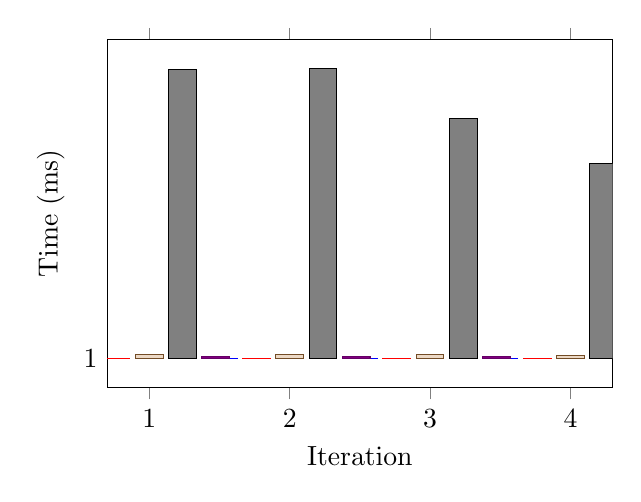
\begin{tikzpicture}
\begin{axis}[ybar, height=6cm, width=8cm, ytick=data, yticklabels={1, 64, 16K, 1M, Max}, xtick=data, xticklabels={1, 2, 3, 4}, xlabel=Iteration, ylabel=Time (ms), legend pos=north west, legend style={at={(0.5,1.03)}, anchor=north, draw=none}]
\addplot coordinates {(1, 0.16) (2, 0.16) (3, 0.16) (4, 0.16)};
\addplot coordinates {(1, 0.42) (2, 0.39) (3, 0.38) (4, 0.34)};
\addplot coordinates {(1, 67.86) (2, 68.10) (3, 56.50) (4, 45.91)};
\addplot coordinates {(1, 4333.76) (2, 4348.58) (3, 3607.68) (4, 2928.72)};
\addplot coordinates {(1, 29.54) (2, 29.43) (3, 35.48) (4, 43.71)};
\end{axis}
\end{tikzpicture}


\end{enumerate}

\section{Results} \label{sec:results}
We can see from the previous graph that the FPGA implementation is able to vastly outperform the CPU implementation, especially for larger data sizes, with just a bit of tweaking and optimization, and shouldn't increase overhead too much for smaller data sizes.
The results also show that the performance of the FPGA implementation is somehow bottlonecked by the system, as the throughput doesn't scale linearly when the PL clock was increased.
We suspect that the culprit is the DDR3 memory, which, as we mentioned before, has a maximum bandwidth of 1050 Mbps. In order to achieve a throughput of 441 Mbps, we actually need to transfer 882 Mbps of data from and to the memory, which is suspiciously close to its maximum bandwidth.


\section{Comparison with Other Hardware} \label{sec:conclusions}
We have successfully proven that the FPGA accelerator is a viable solution for accelerating AES-CTR encryption on the Pynq-Z2 board, 

\printbibliography

\end{document}


